%
% Ra�as de gatos
%

\documentclass[a4paper]{article}

\usepackage{graphicx}
%\usepackage{wrapfig}
\usepackage{subfig}

\graphicspath{{./cats/}}

% Constants
%\newcommand{\DEFAULTWIDTH}{0.3\textwidth}

% Shortcuts
% ...

% Body

\title{Ra\c{c}as de gatos}
\author{Felipe Micaroni Lalli}

\begin{document}

  \maketitle

  \section{Cornish Rex}

  \begin{figure}[h]
    \centering

    \subfloat[][T\'a olhando pra mim?]{
      \label{fig:cornish-rex01}
      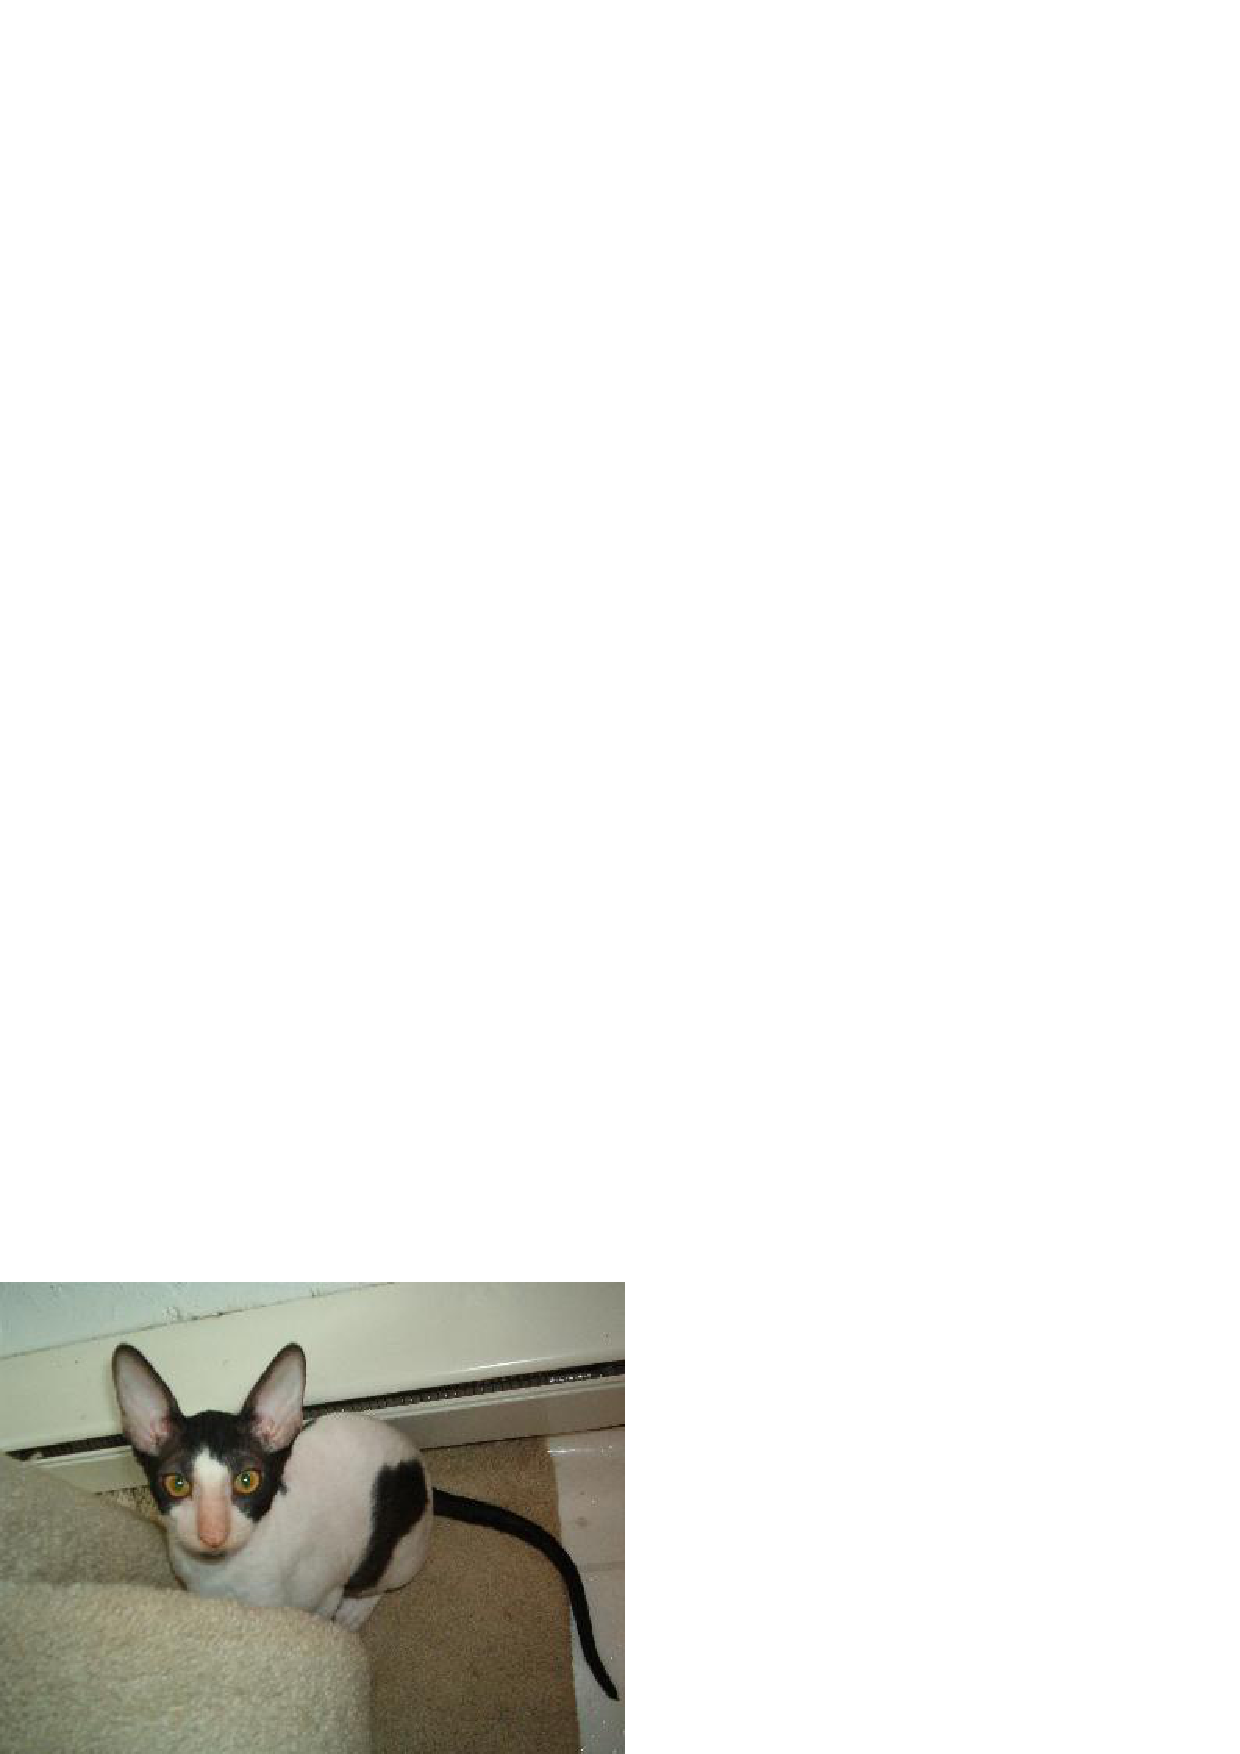
\includegraphics[height=5cm]{cornish-rex01}
    }\subfloat[][Eleg\^ancia de um Cornish Rex]{
      \label{fig:cornish-rex02}
      
\includegraphics[height=5cm]{cornish-rex02}
    }

    \subfloat[][Filhotinho de Cornish Rex]{
      \label{fig:cornish-rex03}
      
\includegraphics[height=5cm]{cornish-rex03}
    }

    \caption{Exemplos de Cornish Rex}
    \label{fig:cornish-rex}
  \end{figure}

  \section{Mau Eg\'ipcio}

  \section{Devon Rex}

  \section{Korat}

  \section{Oriental}

  \section{Sphynx}

  \section{Maine Coon}
  Este \'e o gato gigante.




\end{document}
